\subsection{Gate dell'ADC}

L'ADC a nostra disposizione acquisisce i segnali in ingresso se essi si trovano all'interno di una finestra temporale definita da un segnale logico di \emph{gate}.
Vogliamo sapere se la durata del segnale di gate influisce sulla precisione delle nostre misure.
Variamo la durata del gate dell'ADC e calcoliamo il rapporto $\sigma\!/$\!media per il picco di annichilazione rivelato dal PMT1, modellato come al solito con una gaussiana.

Il risultato di questa misura è in \autoref{fig:gate}, i dati sono in \autoref{tab:gate}.

\begin{figure}[h]
\centering
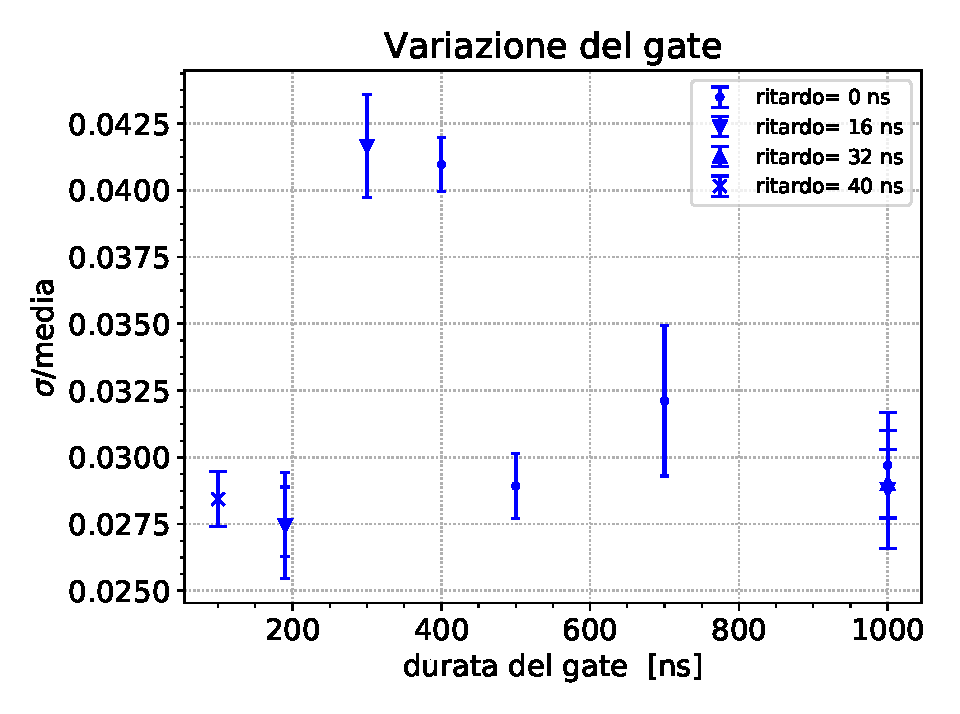
\includegraphics[width=20 em]{immagini/gate}
\caption{Grafico della risoluzione in funzione della durata del gate. Le misure sovrapposte sono state ottenute ritardando il segnale del PMT1.}
\label{fig:gate}
\end{figure}

\begin{table}[h]
\centering
\begin{tabular}{c|c|c|c}
durata (ritardo) [ns] & media [digit] & $\sigma$ [digit] & $\sigma\!/$\!media\\
\hline
 100 &    304.88$\,\pm\,$0.34 &  8.67$\,\pm\,$0.31 & 0.0284 $\,\pm\,$0.0010 \\  
 190 (16)&492.82$\,\pm\,$0.50 & 13.59$\,\pm\,$0.65 & 0.0276 $\,\pm\,$0.0013 \\
 190 &    513.05$\,\pm\,$0.80 & 14.1 $\,\pm\,$1.0 & 0.0274$\,\pm\,$  0.0020 \\
 300 &    307.68$\,\pm\,$0.36 & 12.81$\,\pm\,$0.59 & 0.0416 $\,\pm\,$0.0019 \\
 400 &    344.25$\,\pm\,$0.25 & 14.10$\,\pm\,$0.34 & 0.0410 $\,\pm\,$0.0010 \\
 500 &    524.01$\,\pm\,$0.42 & 15.16$\,\pm\,$0.64 & 0.0289 $\,\pm\,$0.0012 \\
 700 &    482.54$\,\pm\,$0.85 & 15.5 $\,\pm\,$1.4 & 0.0321$\,\pm\,$  0.0028 \\
1000 (16)&539.43$\,\pm\,$0.61 & 16.0 $\,\pm\,$1.1 & 0.0297$\,\pm\,$  0.0020 \\
1000     &553.88$\,\pm\,$0.71 & 15.9 $\,\pm\,$1.2 & 0.0288$\,\pm\,$  0.0022 \\
1000 (32)& 42.68$\,\pm\,$0.41 & 15.75$\,\pm\,$0.69 & 0.0290 $\,\pm\,$0.0013 
\end{tabular}

\caption{Andamento della risoluzione in funzione della durata del gate. I numeri tra parentesi indicano un eventuale ritardo aggiuntivo del PMT1 rispetto al PMT2.}
\label{tab:gate}
\end{table}

Dall'analisi dei dati abbiamo potuto vedere che, fatta eccezione per le misure a \SI{300}{ns} e \SI{400}{ns}, la risoluzione dell'ADC è compatibilmente la stessa.
Abbiamo allora deciso di porre la durata del gate a \SI{550}{ns} perché era il valore usato prima di questa misura.
Questa scelta è poi diventata \SI{1}{\micro s} nel circuito B per evitare problemi derivanti dal jitter dei segnali.